% vapor — a technical monograph: the system as it is, its architecture and its guarantees.
% Build: make technical (lualatex, twice). Separate from monografia/ (the academic record).
\documentclass[11pt,a4paper,open=any,parskip=half,headings=standardclasses,chapterprefix=false,numbers=noenddot]{scrreprt}
\usepackage[margin=2.6cm]{geometry}
% Shared preamble of the technical monograph and the technical slides (LuaLaTeX).
\usepackage{fontspec}
\usepackage{amsmath,amssymb}
\setmonofont{DejaVu Sans Mono}[Scale=0.84]
\newfontfamily\arabicfont[Script=Arabic,Renderer=HarfBuzz,Scale=0.95]{DejaVu Sans}
\newcommand{\ar}[1]{{\arabicfont\textdir TRT #1}}
% LuaTeX has no bidi algorithm: a left-to-right run inside Arabic (a number) is marked by hand
\newcommand{\Lr}[1]{{\textdir TLT #1}}
\usepackage{xcolor}
\definecolor{soot}{HTML}{1E1A14}
\definecolor{brass}{HTML}{B08A3E}
\definecolor{verdigris}{HTML}{3F8F80}
\definecolor{cinnabar}{HTML}{B5432F}
\definecolor{parchment}{HTML}{F4EEE2}
\definecolor{ink}{HTML}{102A30}
\usepackage{booktabs,tabularx,array}
\usepackage{tikz}
\usetikzlibrary{positioning,arrows.meta,fit,calc,shapes.geometric}
\tikzset{
  box/.style={draw=ink, rounded corners=2pt, fill=parchment, align=center, font=\small, inner sep=4pt},
  core/.style={box, fill=brass!25},
  gate/.style={box, fill=verdigris!20},
  edge/.style={-{Stealth[length=2mm]}, ink, thick},
}
\usepackage{listings}
\lstset{basicstyle=\ttfamily\small, columns=fullflexible, keepspaces=true, breaklines=true,
        frame=single, rulecolor=\color{ink!40}, backgroundcolor=\color{parchment},
        xleftmargin=0.5em, xrightmargin=0.5em, aboveskip=0.8em, belowskip=0.8em,
        commentstyle=\color{verdigris}, keywordstyle=\color{cinnabar}}
\setlength{\emergencystretch}{3em}
\newcommand{\vapor}{\textsf{vapor}}
\newcommand{\Q}{\mathbb{Q}}

\usepackage[hidelinks]{hyperref}
\addtokomafont{disposition}{\color{ink}}
\RedeclareSectionCommand[beforeskip=0pt,afterskip=1.6em]{chapter}
\usepackage{microtype}
\renewcommand{\arraystretch}{1.18}

\title{\Huge\bfseries\color{ink} vapor\\[0.6em]
       \LARGE\mdseries A certified tensor compiler and the laboratory built on it\\[0.4em]
       \large Architecture, semantics and guarantees}
\author{João Phamata}
\date{Technical monograph — version 0.17}

\begin{document}
\maketitle
\begin{abstract}
\vapor{} is a compiler and runtime for tensor programs, written in Elixir on the BEAM with a small
native worker in Zig, and a laboratory of tools built on top of it. Its organising principle is that
every result carries what is needed to judge it. Tensor programs compile to machine code for x86-64
(AVX2, AVX-512), AArch64, RISC-V with the vector extension and Vulkan, and under the canonical policy
produce the same bits on all of them and on an exact binary32 oracle. Register allocation is checked by
a verifier proved correct in Lean~4 and extracted to Elixir. A six-rung verification ladder ends in an
Ed25519 certificate that independent nodes can reproduce byte for byte and co-sign. Models enter
through an airlock that separates the function a network computes from the way a family spells it;
network access enters through a second airlock that only the person can open. Around the core sit
deciders whose answers come with independently checked certificates (exact linear and integer
programming, SAT with DRUP proofs, Gröbner bases, causal identification, polynomial positivity, circuit
equivalence), a bilingual language of decided claims, a search engine whose results are re-verified,
and an evidence discipline in which every quality check is paired with a control. This monograph
describes the system as it is, its architecture, the invariants each component keeps, how they are
checked, and the limits that remain.
\end{abstract}

\tableofcontents

\chapter{Introduction}

\section{What the system is}

\vapor{} has two parts that share one discipline.

The first is a \textbf{compiler and runtime for tensor programs}. A program is a term of a small free
algebra (element-wise operations, contractions, reductions, the operators of modern neural networks)
whose meaning is fixed by an exact reference implementation, the \emph{oracle}. The compiler lowers a
program to a portable kernel IR, allocates registers without spilling, and encodes machine code for
four instruction sets and for Vulkan compute shaders. The runtime executes that code in a separate,
sandboxed process, keeps model weights in content-addressed shared memory, serves models through an
OpenAI-compatible interface and records a receipt for every answer.

The second is a \textbf{laboratory}: deciders, languages, search, numerical workbenches, statistical
tools, document readers and desks for engineering and finance, all reachable from one command-line
interpreter, a browser console, an MCP server for agents, a language server for editors, and a small
editor of its own.

What the two share is the rule that a result is never just a value. A compiled kernel comes with the
evidence that it computes the oracle's bits; an \emph{optimal} integer program comes with a
branch-and-bound tree that separate code checks; a refuted conservation law comes with the point that
refutes it; a statistical claim comes with a control that a broken implementation would have passed.

\section{Three properties}

Three properties run through every chapter.

\paragraph{Determinism.} Under the \emph{canonical} numerical policy, a program produces the same bits
on every substrate: x86-64 with AVX2 or AVX-512, AArch64 with NEON, RISC-V with RVV (native or
interpreted), Vulkan (on any driver) and the oracle. The bits also do not depend on the number of
threads, on how many sequences share a decoding step, on where the key--value cache lives, or on which
replica serves a request. Parallelism is drawn from independent outputs, never from reassociating a sum
(Chapter~\ref{ch:semantics}).

\paragraph{Certification.} Wherever a claim can be checked by a procedure simpler than the one that
produced it, the system ships the certificate and the checker. Register allocations are revalidated by
a checker proved sound in Lean~4. Kernels climb a ladder of differential checks that ends in a signed,
reproducible certificate. Deciders return witnesses, Farkas vectors, DRUP proofs or hedges, and each is
checked by code that shares nothing with the search (Chapters~\ref{ch:verification}
and~\ref{ch:deciders}).

\paragraph{Containment.} Nothing generated runs inside the BEAM: there are no NIFs. Machine code runs in
a static, libc-free worker under seccomp, with W\^{}X pages and a watchdog. Work on untrusted input runs
under one containment primitive, the \emph{hermetic seal}, which caps memory (on-heap and off-heap) and
time. Models enter only through the model airlock; bytes from the network enter only through the
network airlock, and only a person can open it (Chapters~\ref{ch:models} and~\ref{ch:network}).

\section{How to read this document}

Chapter~\ref{ch:overview} gives the layers and the trust boundaries. Chapters~\ref{ch:semantics}
to~\ref{ch:verification} describe the core: the algebra and its numerical semantics, the compiler, the
runtime and the verification ladder. Chapters~\ref{ch:models} and~\ref{ch:network} describe the two
airlocks. Chapters~\ref{ch:deciders} and~\ref{ch:languages} describe the certified deciders and the
languages built on them. Chapter~\ref{ch:evidence} describes how quality is measured and how the test
suite is organised, Chapter~\ref{ch:interfaces} the interfaces, and Chapter~\ref{ch:limits} what the
system does not do. The appendix maps components to modules.

Every statement of fact in this document corresponds to a test or a check in the repository, named in
the system's own documents (\texttt{docs/}); this monograph gives the architecture and leaves the
contestation commands to them.

\chapter{System overview}\label{ch:overview}

\section{Layers}

Figure~\ref{fig:layers} shows the layers. Each layer uses the ones below it and adds no trust to them:
what a layer produces is either a certified program for the core or canonical data.

\begin{figure}[h]
\centering
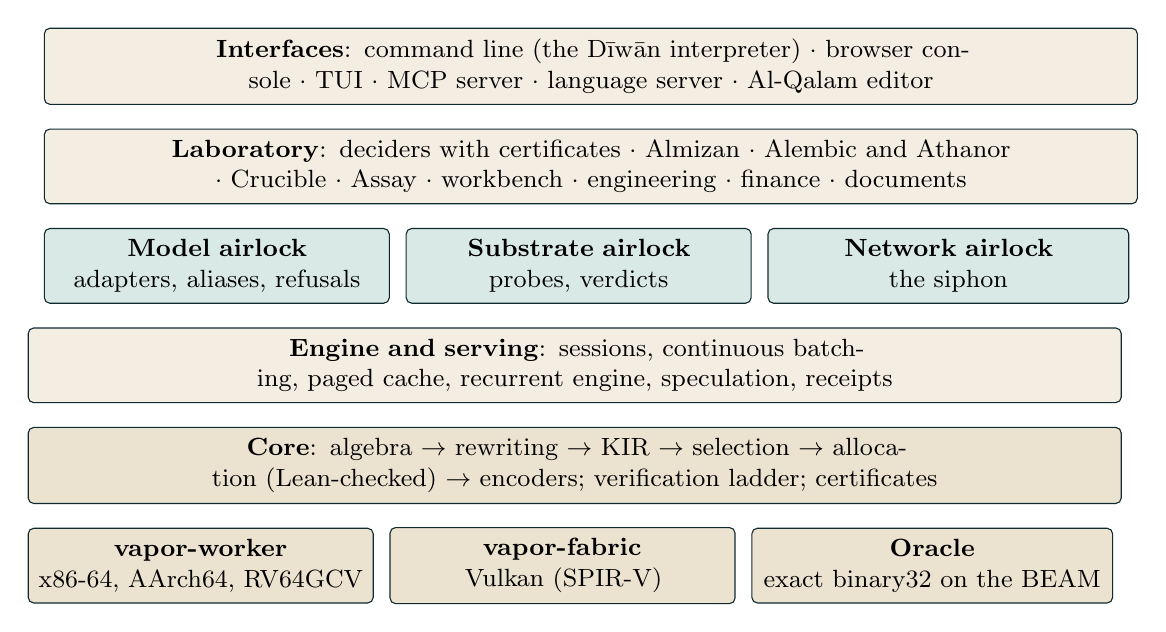
\begin{tikzpicture}[node distance=3mm, every node/.style={minimum height=8mm}]
  \node[box, text width=13.6cm] (ifc) {\textbf{Interfaces}: command line (the Dīwān interpreter) $\cdot$ browser console $\cdot$ TUI $\cdot$ MCP server $\cdot$ language server $\cdot$ Al-Qalam editor};
  \node[box, text width=13.6cm, below=of ifc] (lab) {\textbf{Laboratory}: deciders with certificates $\cdot$ Almizan $\cdot$ Alembic and Athanor $\cdot$ Crucible $\cdot$ Assay $\cdot$ workbench $\cdot$ engineering $\cdot$ finance $\cdot$ documents};
  \node[gate, text width=4.1cm, below=of lab.south west, anchor=north west] (mair) {\textbf{Model airlock}\\adapters, aliases, refusals};
  \node[gate, text width=4.1cm, right=2mm of mair] (sair) {\textbf{Substrate airlock}\\probes, verdicts};
  \node[gate, text width=4.3cm, right=2mm of sair] (nair) {\textbf{Network airlock}\\the siphon};
  \node[box, text width=13.6cm, below=of sair.south, anchor=north, xshift=-0.05cm] (eng) {\textbf{Engine and serving}: sessions, continuous batching, paged cache, recurrent engine, speculation, receipts};
  \node[core, text width=13.6cm, below=of eng] (cmp) {\textbf{Core}: algebra $\to$ rewriting $\to$ KIR $\to$ selection $\to$ allocation (Lean-checked) $\to$ encoders; verification ladder; certificates};
  \node[core, text width=4.1cm, below=of cmp.south west, anchor=north west] (wk) {\textbf{vapor-worker}\\x86-64, AArch64, RV64GCV};
  \node[core, text width=4.1cm, right=2mm of wk] (fb) {\textbf{vapor-fabric}\\Vulkan (SPIR-V)};
  \node[core, text width=4.3cm, right=2mm of fb] (or) {\textbf{Oracle}\\exact binary32 on the BEAM};
\end{tikzpicture}
\caption{Layers. The airlocks are the only ways in for models, substrates and network bytes.}
\label{fig:layers}
\end{figure}

\paragraph{The core} turns a term of the algebra into machine code and evidence. It is about ten
thousand lines of Elixir (algebra, compiler, kernel IR, encoders, verification, runtime), plus the
code extracted from Lean and the native worker.

\paragraph{The engine} runs compiled model programs in resident sessions: one compilation, many steps,
weights mapped once. It schedules many sequences into one step without changing any sequence's bits.

\paragraph{The airlocks} are the boundaries through which outside things enter. A checkpoint must be
claimed by an adapter that writes its function in the algebra; a substrate must pass numerical probes
before it receives canonical programs; a byte from the network must come through a fetcher that the
person declared and ran.

\paragraph{The laboratory} holds tools whose answers carry their evidence. Some compile to the core
(a Monte Carlo pricer whose generator is written as algebra terms, so the same bits come out on every
substrate); most inherit only its canonical encodings, Merkle trees and the discipline of independent
checking.

\section{Trust boundaries}

\begin{table}[h]
\centering\small
\begin{tabularx}{\textwidth}{@{}lX@{}}
\toprule
boundary & what crosses it, and what keeps it \\
\midrule
BEAM $\leftrightarrow$ native code & framed messages on stdio ({\ttfamily\{packet, 4\}}); no NIF is loaded (a test forbids it); a crash, an illegal instruction or a timeout kills the worker process, which is restarted, and the next unit runs \\
worker $\leftrightarrow$ kernel & seccomp-BPF allow-list, \texttt{PR\_SET\_NO\_NEW\_PRIVS}, W\^{}X code pages, a \texttt{SIGALRM} watchdog \\
job $\leftrightarrow$ host & the hermetic seal: a process with a heap cap that counts off-heap binaries, and a deadline \\
checkpoint $\leftrightarrow$ engine & the model airlock: claimed by an adapter, every tensor accounted for, configuration keys that change the mathematics read or refused by name \\
substrate $\leftrightarrow$ dispatcher & the substrate airlock: probes classify a substrate as canonical, within an envelope, or refused \\
network $\leftrightarrow$ system & the siphon: only fetchers the person declares, run by the person; an agent can only queue a request \\
agent $\leftrightarrow$ world & effect classes (\texttt{pure}, \texttt{observe}, \texttt{act}), grants fixed in the agent's digest, a write-ahead journal \\
\bottomrule
\end{tabularx}
\caption{Trust boundaries and what holds each.}
\end{table}

The trusted base is the BEAM, the Linux kernel, the IEEE-754 standard model of rounding (from which the
error bounds are proved), the printer of the Lean extractor (about two hundred lines), and the Vulkan
driver, which runs in its own process.

\section{Size}

\begin{table}[h]
\centering\small
\begin{tabular}{@{}lr@{}}
\toprule
component & lines \\
\midrule
Elixir, all of \texttt{lib/} (379 files, 425 modules) & 101{,}000 \\
\quad of which the core (algebra, compiler, KIR, encoders, verification, runtime) & 10{,}400 \\
native worker and Vulkan daemon (Zig, \texttt{native/src}) & 4{,}700 \\
Lean~4 proofs and extractor (82 theorems, no \texttt{sorry}, no \texttt{axiom}) & 1{,}500 \\
tests (Elixir, and the Python and Node scripts of the differential tiers; 159 files) & 27{,}000 \\
\bottomrule
\end{tabular}
\caption{Size of the system. The native binaries are 330--360\,KB each; the BEAM application has no
dependencies outside OTP and Elixir.}
\end{table}

A full build takes about thirty seconds on two virtual CPUs. The application declares no Hex
dependency: JSON, CBOR, SHA-256 trees, Ed25519, safetensors, GGUF, PNG, JPEG, PDF and the HTTP server are
implemented in the tree or taken from OTP.

\chapter{The algebra and its numerical semantics}\label{ch:semantics}

\section{Programs are terms}

A program is a term of \texttt{Vapor.Algebra.Term}, a \emph{symbolic} free algebra: every operator is a
name whose meaning is fixed by the oracle (\texttt{Vapor.Runtime.Oracle}), never an embedded closure.
That is what makes a term compilable to machine code and comparable across substrates.

\begin{itemize}
\item \textbf{Generators}: inputs and constants; element-wise operations (\texttt{add}, \texttt{sub},
  \texttt{mul}, \texttt{fma}, \texttt{neg}, \texttt{relu}, the canonical transcendental functions, the
  comparison-select \texttt{sel(a,b,x,y)} $= a<b\ ?\ x : y$); contractions (\texttt{linear}$(x,w) =
  xw^{\mathsf T}$, grouped and masked variants, 4-bit and int8 matrices); reductions that keep rank; and
  the operators of neural networks (\texttt{gather\_row}, \texttt{rope}, \texttt{kv\_write} and
  \texttt{attention} with an explicit scale, contiguous and paged, \texttt{sample}).
\item \textbf{Semi-dynamic dimensions} \texttt{\{:dyn, :S, max\}}: every bound is established at the
  maximum, and monotonicity lemmas proved in Lean carry the certificate to every extent $S \le
  \textit{max}$.
\item \textbf{Recurrent programs} declare state feedback (\texttt{state: [h: :h\_next]}): the whole
  loop runs in the worker behind one crossing from the BEAM, the state never leaves the worker, and
  outputs stream per step.
\end{itemize}

Numerical data live in contiguous binaries (\texttt{Vapor.Tensor}); random access uses tuples.

\section{Exact binary32 on the BEAM}

\texttt{Vapor.F32} implements binary32 exactly: values are bit patterns; \texttt{add}, \texttt{sub} and
\texttt{mul} go through binary64 and one rounding (correct, since $53 \ge 2\cdot 24 + 2$); \texttt{fma}
is computed in dyadic rationals with a single rounding, round-to-nearest-even, gradual underflow and
overflow to infinity. It agrees with the hardware on 800{,}000 operations including subnormals and
signed zeros. The oracle is built on it.

\section{Two policies}

\begin{table}[h]
\centering\small
\begin{tabularx}{\textwidth}{@{}lXX@{}}
\toprule
policy & semantics & guarantee \\
\midrule
\texttt{:canonical} & multiply and add rounded separately; every reduction in one fixed 16-lane tree
($r_8 \to r_4 \to r_2 \to r$); division correctly rounded; transcendental functions as fixed
micro-programs & identical bits on x86-64, AArch64, RVV, the interpreter, Vulkan and the oracle \\
\texttt{:fast} & fused multiply--add where the operator allows & every output inside a rigorous error
envelope on every substrate \\
\bottomrule
\end{tabularx}
\caption{Numerical policies.}
\end{table}

The central idea is that reproducibility does not require slowness when parallelism comes from
independent outputs. Each row of a matrix--vector product has exactly sixteen accumulators reduced in
the fixed tree, whatever the vector width; throughput comes from processing several rows per iteration
(chosen by the register allocator per instruction set), which changes no bit.

Under the canonical policy $+$, $-$, $\times$ and $\div$ are IEEE operations on every substrate (with
the GPU convention of flushing subnormals for division: DAZ/FTZ). Division is computed by Markstein's
method with Dekker's exact residual and no fused operation; the logarithm is within one ulp of the
correctly rounded value; the other transcendental functions are within one or two ulps, identical
everywhere. Tables that must be exact, such as rotary position frequencies, are computed by a
correctly rounded routine (\texttt{Vapor.CR}, Ziv's strategy).

\paragraph{Semantics version.} The bits of a program are a function of its terms \emph{and} of the
definition of the canonical functions. Certificates record \texttt{Vapor.Canon.version/0}, so a change
in a canonical function cannot silently change what a certificate means.

\section{The error envelope}

For the fast policy and for substrates that are not canonical, \texttt{Vapor.Verify.Envelope} computes,
for every output, the exact real value and a rigorous bound valid for \emph{any} conforming substrate
(correct rounding, fused or unfused multiply--add, any reduction order, gradual underflow or
flush-to-zero), in exact dyadic rationals. Contractions over exact inputs take the Wilkinson form
$\gamma_n S + a$, decided by \texttt{within\_envelope/4} (extracted from Lean); other operations use
running error analysis. The verifier never rounds; bounds are only ever shortened upward. The Higham
form of $\gamma_n$, a bound on products of $(1+\delta_i)$, is proved in Lean from the standard model
$\mathrm{fl}(x \mathbin{\mathrm{op}} y) = (x \mathbin{\mathrm{op}} y)(1+\delta)$, $|\delta| \le 2^{-24}$.

\section{Rewriting without error}

\texttt{Vapor.Compile.Rewrite} admits only identities that hold bit for bit over all of IEEE-754,
signed zeros included: $\mathrm{neg}(\mathrm{neg}\,x) \to x$, $x\cdot 1 \to x$, $x + (-0) \to x$,
$x - (+0) \to x$, but not $x + (+0) \to x$, because $(-0) + (+0) = +0$. Constant folding evaluates the
declared semantics themselves. Rewriting therefore has error $\varepsilon = 0$ by construction.

\chapter{The compiler}\label{ch:compiler}

\begin{figure}[h]
\centering
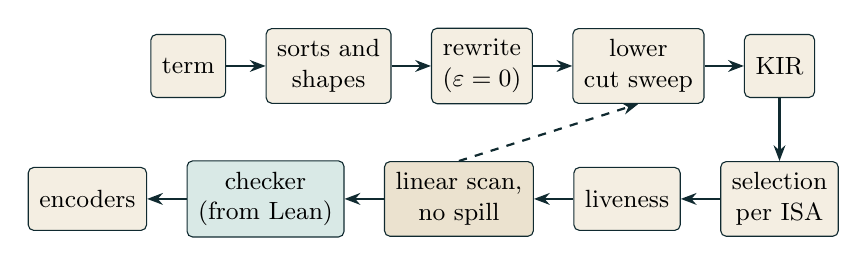
\begin{tikzpicture}[node distance=5mm and 5mm, every node/.style={minimum height=8mm}]
  \node[box] (t) {term};
  \node[box, right=of t] (s) {sorts and\\shapes};
  \node[box, right=of s] (r) {rewrite\\($\varepsilon=0$)};
  \node[box, right=of r] (l) {lower\\cut sweep};
  \node[box, right=of l] (k) {KIR};
  \node[box, below=8mm of k] (sel) {selection\\per ISA};
  \node[box, left=of sel] (live) {liveness};
  \node[core, left=of live] (ra) {linear scan,\\no spill};
  \node[gate, left=of ra] (chk) {checker\\(from Lean)};
  \node[box, left=of chk] (enc) {encoders};
  \draw[edge] (t)--(s); \draw[edge] (s)--(r); \draw[edge] (r)--(l); \draw[edge] (l)--(k);
  \draw[edge] (k)--(sel); \draw[edge] (sel)--(live); \draw[edge] (live)--(ra); \draw[edge] (ra)--(chk); \draw[edge] (chk)--(enc);
  \draw[edge, dashed] (ra.north) -- (l.south);
\end{tikzpicture}
\caption{The compilation pipeline. An allocation that runs out of registers is never spilled: the
compiler goes back (dashed) and retries with a smaller group factor, fewer rows per iteration, or a cut of the fused region.}
\end{figure}

\section{A portable kernel IR}

Kernels (\texttt{Vapor.KIR.Kernels}: fused element-wise strips, reductions, matrix--vector products in
f32, bf16 and 4-bit formats, int8 matrix products, and the model operators) are written once over
virtual registers with \emph{types}: \texttt{:strip}, \texttt{:f16l} (sixteen f32 lanes),
\texttt{:i32acc} and others. Each backend sizes the types. The \textbf{group factor} $g$ generalises
the RVV register-group multiplier (LMUL) to every instruction set: an AVX2 strip with $g=4$ is four
\texttt{ymm} registers in lockstep, an RVV strip with $g=8$ is an \texttt{m8} group.

\begin{table}[h]
\centering\small
\begin{tabular}{@{}lllll@{}}
\toprule
type & RVV & AVX2 & AVX-512 & NEON \\
\midrule
\texttt{:strip} & m$g$ & $g$ ymm & $g$ zmm & $g$ q \\
\texttt{:f16l} & m4, vl$=16$ & 2 ymm & 1 zmm & 4 q \\
\texttt{:i32acc} & m$4g$ & $g$ ymm & $g$ zmm & 2 q \\
\bottomrule
\end{tabular}
\caption{One kernel IR, four register files.}
\end{table}

Selection happens \emph{before} allocation, as in production compilers. Lane-wise instructions are
emitted as bundles (one allocation unit), so a destination can reuse a source register that dies at
that point. On AVX-512, strip tails are one masked pass (\texttt{bzhi} into mask registers, masked loads
and stores only) instead of a scalar loop, and four-byte constants use embedded broadcast; the
reduction tree is lane for lane the same as AVX2's, so the bits are the same.

\section{Allocation without spill, checked}

\texttt{Vapor.KIR.Liveness} computes liveness by fixed point over the control-flow graph (values live on
a back edge cover the whole loop), with early-clobber constraints for the overlap rules of RVV's
widening instructions. \texttt{Vapor.KIR.RegAlloc} is a linear scan with aligned blocks of one, two,
four or eight registers.

There is no spill path. When registers run out, the allocator returns the pressure point, and the
compiler tries a smaller group factor, then fewer rows per iteration for the 4-bit products, then a
cut of the fused region at that point. Every accepted allocation is revalidated by
\texttt{check\_alloc/3}, which is extracted from Lean together with its soundness theorem
(\texttt{checkAlloc\_sound}): groups are aligned, inside the register file, outside the reserved
registers, and no two simultaneously live values share a register. Every emitted region is therefore
free of spill and clobber by construction, not by trust in the heuristic.

\section{Encoders}

\begin{table}[h]
\centering\small
\begin{tabularx}{\textwidth}{@{}lX@{}}
\toprule
target & encoding \\
\midrule
x86-64 (AVX2, AVX-512) & REX, three-byte VEX, EVEX (always \texttt{disp32}), ModR/M, SIB; System~V ABI, callee-saved registers saved only when used \\
AArch64 (NEON) & A64 words; AAPCS64, \texttt{x18} never allocated \\
RV64GCV & \texttt{vtype} fields, vector loads and stores with width fields, static round-to-nearest for scalar FP; full psABI; long branches as an inverted branch over a \texttt{jal} \\
SPIR-V (Vulkan) & a symbolic assembler that interns types and constants and orders the logical sections; \texttt{NoContraction} on every multiply and add under the canonical policy \\
MSL, StableHLO & emitted for Metal and for PJRT devices, and admitted only through the substrate airlock \\
\bottomrule
\end{tabularx}
\caption{Encoders. The product never calls an assembler.}
\end{table}

The tests validate every emitted instruction (every kernel constructor, in every backend, at every
group factor and policy) against GNU binutils, and every SPIR-V module against \texttt{spirv-val}.
Those tools are used only to check; the product encodes bytes itself.

\section{Cost model}

The arbiter predicts the time of a schedule on a substrate as
\[
  t = \sum_{\text{loops}} \max\!\left(\frac{F}{\pi}, \frac{Q}{\beta}, \frac{I}{\iota}\right) + \text{overheads},
\]
with floating-point work $F$ and bytes $Q$ counted from the schedule and $I$ the static count of
instructions in each hot loop as emitted, times its iterations. The third ceiling makes the model
honest: the 4-bit matrix--vector product is bound by instruction issue (about 1.1 instructions per
weight), not by bandwidth, and a two-ceiling model misses it by a factor of about five. Profiles are
declared per vendor; the dispatch decision is the argmin of the predicted time, taken on each node from
the certified work and the node's own profile.

\chapter{Substrates and the runtime}\label{ch:runtime}

\section{The worker}

\texttt{vapor-worker} is a static Zig executable with no libc. At start-up (\textsc{hello}) it fixes the
number of threads; the thread pool and the event counters (\texttt{perf\_event\_open}: cycles,
instructions and cache events when a PMU exists; task clock, page faults and context switches always)
are created \emph{before} the seccomp filter, which is installed with \texttt{TSYNC} on every thread.
Each call carries a \emph{partition descriptor} (a count argument, a grain, pointers that advance per
unit, per-thread scratch, an optional guard) and the worker splits the units among threads. Because the
units are independent rows, the result is the same for one thread or many.

Code runs in one of two modes. \textbf{Native}: the machine code is copied to a writable page, the page
is made read--execute (W\^{}X), the instruction cache is synchronised where the architecture needs it,
and the kernel is called as \texttt{void k(const uint64\_t *args)}. \textbf{Emulated}: RV64GCV code is
interpreted by \texttt{rvemu.zig}, which checks every memory access against the bound buffers and every
fetch against the code, and turns an unknown instruction into an error with its address and word. The
interpreter implements RVV~1.0 faithfully (round-to-nearest, fused \texttt{vfmacc}, canonical NaN,
NaN-boxing, group alignment, \texttt{vill}), with a \emph{poison} mode that writes ones into
tail- and mask-agnostic elements, proving that kernels do not depend on them, and a configurable VLEN
from 128 to 512 bits.

Containment is a seccomp-BPF allow-list (read, write, openat, close, lseek, mmap, munmap, mprotect,
clock\_gettime, setitimer, signals, exit; the architecture is audited),
\texttt{PR\_SET\_NO\_NEW\_PRIVS}, and a \texttt{SIGALRM} watchdog for native code that does not finish.
The tests provoke all four failure classes (\texttt{SIGILL}, \texttt{SIGSEGV}, \texttt{SIGALRM},
\texttt{SIGSYS}); in each, only the worker dies, the BEAM process that owns it reports the signal,
restarts it, and the next unit runs.

\section{The Vulkan daemon}

\texttt{vapor-fabric} drives Vulkan compute through hand-written bindings (libc only for the loader's
\texttt{dlopen}): instance, physical device with a compute queue, logical device, buffers, shader modules
from the SPIR-V emitted by the BEAM, pipelines with push constants, descriptor sets, one command buffer
per run with barriers, per-iteration windows and state copies, submission with a fenced deadline, and
readback. A driver crash or a lost device kills only the daemon. Its plans are self-contained, so a
restarted daemon needs no replay.

\section{One protocol}

Both processes speak the same framing: \texttt{\{packet, 4\}} frames on standard I/O (big-endian
length, little-endian fields), so a process that dies in the middle of a frame cannot desynchronise the
BEAM.

\begin{table}[h]
\centering\small
\begin{tabularx}{\textwidth}{@{}llX@{}}
\toprule
frame & code & content \\
\midrule
\textsc{hello} & 1 & flags, threads $\to$ architecture, sandbox state, version, threads \\
\textsc{run} & 2 & mode, VLEN, flags, fuel, deadline, code, buffers (inline or mapped files), calls with arguments and partition descriptors, iterations, streamed emissions, copies, returns \\
\textsc{emit} & 3 & per-iteration output, streamed \\
\textsc{done} & 4 & elapsed time, retired instructions, counters, returned buffers \\
\textsc{err} & 5 & code, program counter, instruction word, message \\
\textsc{open}, \textsc{step}, \textsc{close} & 6--8 & resident sessions: weights mapped once, state kept between steps, each step writing only its inputs and returning only the requested outputs, with optional state copies inside the worker \\
\bottomrule
\end{tabularx}
\caption{The worker protocol. Tables are sized by the frame itself, so a hostile count cannot allocate
more than the frame describes.}
\end{table}

\section{Memory}

Weights of 64\,KiB or more are written once to \texttt{/dev/shm/vapor-<sha256>} (content addressed,
atomic write) and mapped copy-on-write by every worker; the Vulkan daemon imports them without copy
through \texttt{VK\_EXT\_external\_memory\_host} when the device offers it. Replicas and restarts map the
same files, so $n$ workers serving one model occupy one copy in the page cache. Weights can stay in
bfloat16: the kernels widen sixteen weights exactly on load, so the result is bit for bit that of the
f32 program over the rounded values. Per-token inputs are windows into one buffer; state feedback
($h \leftarrow h_{\text{next}}$) is a copy declared in the plan.

\section{Dispatch and failover}

\texttt{Vapor.Runtime.Dispatch} tries the arbiter's choice and walks down the chain
\[
\text{fabric} \to \text{host AVX-512} \to \text{host base ISA} \to \text{RVV interpreter} \to \text{oracle},
\]
recording the reason for each step. Under the canonical policy every link computes the same bits, so
rerouting never changes an answer.

\section{Parallelism without changing bits}

\begin{table}[h]
\centering\small
\begin{tabularx}{\textwidth}{@{}lXl@{}}
\toprule
form & where & invariant \\
\midrule
SIMD & AVX2, AVX-512, NEON, RVV (VLEN 128--512), SPIR-V & same bits as the oracle \\
instruction-level & $R$ rows per iteration in matrix--vector products, chosen by the allocator & same \\
threads & the worker's pool; decode attention split by key--value head & 1 thread $=$ $n$ threads \\
continuous batching & decode and prefill chunks in one step & a sequence alone $=$ in a batch \\
paged cache & paged key--value writes and attention over a block table & paged $=$ contiguous \\
replicas & one compilation, shared weight pages, shortest queue & same answer from any replica \\
speculation & a draft proposes, the target verifies $k{+}1$ rows in one step & output $=$ the target's \\
GPU & SPIR-V for every model operator & fabric $=$ oracle \\
\bottomrule
\end{tabularx}
\caption{Every form of parallelism draws on independent outputs.}
\end{table}

Speculative decoding needs no further correctness argument: the $k{+}1$-row verification step is
bit-identical to $k{+}1$ single steps by batch invariance, so the output equals the target's greedy
decoding whatever the draft, and the draft only changes the number of steps. Block drafters and tree
drafts are degenerate and general cases of the same rule.

\section{The engine and serving}

\texttt{Vapor.Engine} serves compiled models in resident sessions with continuous batching, a paged
key--value cache, replicas and cancellation: the engine monitors the process that asked for each
sequence, and a sequence whose requester dies leaves the batch at the next step boundary without
changing the bits of the others. Recurrent models (Mamba, Mamba-2, the delta-rule hybrid of
Chapter~\ref{ch:models}) run as step programs whose state stays in the worker. The HTTP server speaks
the OpenAI chat and completion protocols with streaming, and every response carries a receipt, the
canonical digest of model, prompt tokens, parameters and generated tokens. Constrained decoding
(\texttt{Vapor.Grammar}) restricts generation to a grammar derived from a JSON Schema, a regular
expression or a tool's declared arguments, with the invariant that no accepted prefix is a dead end.

\chapter{Verification and certificates}\label{ch:verification}

\section{The ladder}

A program is certified by climbing six rungs. Each rung checks something the previous one cannot.

\begin{table}[h]
\centering\small
\begin{tabularx}{\textwidth}{@{}clX@{}}
\toprule
rung & establishes & how \\
\midrule
1 & sorts, shapes, feedback & \texttt{Program.check/1} \\
-- & exact rewriting & only identities valid over all of IEEE-754 \\
2 & admission & the allocation accepted by the extracted checker on \emph{every} instruction set; int8 contractions free of wrap-around at the maximum extents (\texttt{admissible/3}); SPIR-V limits \\
3 & adjoint identity & $\langle Wx, v\rangle = \langle x, W^{\mathsf T}v\rangle$ between the compiled kernel and the exact transpose: catches layout and transposition errors \\
4 & differential oracle & each CPU substrate equal to the exact oracle, bit for bit \\
5 & parity and envelope & equal FNV-1a digests across substrates; every output inside the envelope \\
6 & proof-carrying code & an Ed25519 certificate with a quorum of co-signatures \\
\bottomrule
\end{tabularx}
\caption{The verification ladder.}
\end{table}

\section{The certificate}

The payload holds the SHA-256 of the program, of each machine-code blob and of each SPIR-V module; the
digest of the Lean sources of the checkers; the evidence of each rung; and the \emph{counted work}
(floating-point operations, bytes, instructions per instruction set). It holds nothing that depends on
the host: no timings and no dispatch decision. Independent nodes that redo the ladder therefore produce
payloads identical byte for byte and can co-sign them (\texttt{Certificate.cosign/3});
\texttt{verify/3} requires a quorum of valid signatures from distinct trusted keys. A bundle packages
artefacts and certificate, and an edge node checks signatures and hashes in about two milliseconds and
runs the code without redoing the ladder.

\section{What is proved in Lean}

The Lean~4 development uses the core library only, with no \texttt{axiom} and no \texttt{sorry}. It
proves, among its 82 theorems:

\begin{itemize}
\item in $\mathbb{Z}/2^{32}\mathbb{Z}$: associativity and commutativity, that wrapping is a homomorphism,
  and that \emph{every} reduction tree with a wrapping adder computes the exact value when
  $K\cdot\max|A|\cdot\max|B| < 2^{31}$, for any permutation of the leaves (\texttt{integer\_parity});
  monotonicity of admissibility;
\item for memory banks: coprime strides are injective on the lanes (\texttt{bank\_injective}), and the
  closed-form padding for $2^m$ banks is sufficient and minimal;
\item for recurrences: the affine monoid is associative with neutral element $(1,0)$, composition is
  sequential application, and segmented lifting is associative for any monoid;
\item the soundness of the allocation checker (\texttt{checkAlloc\_sound});
\item the exact envelope decision and its monotonicity in the extent; Higham's bound on products of
  $(1+\delta_i)$;
\item the depth of Estrin's evaluation scheme against Horner's, computed over the tree.
\end{itemize}

\section{Extraction}

The extractor (\texttt{lake exe vapor-extract}) reads the \emph{elaborated} definitions (the same terms
the theorems speak about) and prints Elixir, failing on any construct outside its fragment. The
extracted functions are \texttt{check\_alloc}, \texttt{admissible}, \texttt{wrap\_s32},
\texttt{pad\_stride}, \texttt{bank\_of}, \texttt{affine\_op}, \texttt{seg\_affine} and
\texttt{within\_envelope}. Lean computes more than 480 conformance vectors that the extracted code must
reproduce, and the generated module carries the digest of the Lean sources, which a test checks without
needing the Lean toolchain. Extraction happens at build time: production never runs Lean.

\section{What is tested and what is trusted}

Tested but not proved: the encoders (against binutils and \texttt{spirv-val}, and by execution under
QEMU and lavapipe), the RVV interpreter against QEMU at VLEN 128, 256 and 512, bit-for-bit equality
across substrates, and fault containment. Trusted: the BEAM and the Linux kernel, the extractor's
printer and its six-line prelude, the IEEE-754 standard model, and the Vulkan driver, contained in its
own process.

\chapter{Models: the airlock}\label{ch:models}

\section{The contract, not the family}

A program in the algebra is self-describing: its inputs, outputs and state are typed terms. What the
core needs to know about a model is therefore the \emph{shape of its program}, not its family. The model
airlock (\texttt{Vapor.Lock}) is the only place where a family is known. Inside, there is only a
\texttt{Vapor.Lock.Spec}, the contract, and a program checked against it.

\begin{figure}[h]
\centering
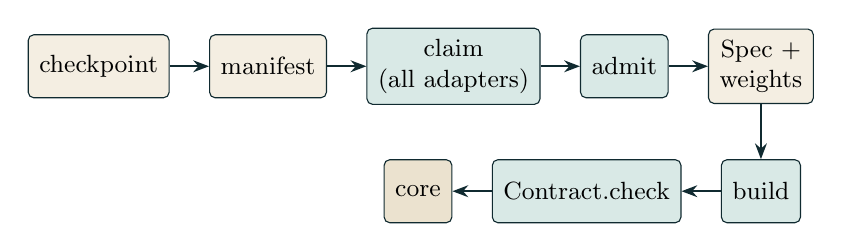
\begin{tikzpicture}[node distance=5mm, every node/.style={minimum height=8mm}]
  \node[box] (ck) {checkpoint};
  \node[box, right=of ck] (mf) {manifest};
  \node[gate, right=of mf] (cl) {claim\\(all adapters)};
  \node[gate, right=of cl] (ad) {admit};
  \node[box, right=of ad] (sp) {Spec +\\weights};
  \node[gate, below=7mm of sp] (bd) {build};
  \node[gate, left=of bd] (ct) {Contract.check};
  \node[core, left=of ct] (co) {core};
  \draw[edge] (ck)--(mf); \draw[edge] (mf)--(cl); \draw[edge] (cl)--(ad); \draw[edge] (ad)--(sp);
  \draw[edge] (sp)--(bd); \draw[edge] (bd)--(ct); \draw[edge] (ct)--(co);
\end{tikzpicture}
\caption{Admission. A defective adapter is stopped at the boundary, not inside the engine.}
\end{figure}

\begin{table}[h]
\centering\small
\begin{tabularx}{\textwidth}{@{}lXXl@{}}
\toprule
contract & inputs & outputs & state \\
\midrule
\texttt{:causal\_lm} & tokens and positions (and, by option, sampling, a block table, a slot, soft tokens) & logits and/or hidden rows & paired $\{x, x_{\text{next}}\}$ of equal sorts \\
\texttt{:encoder} & rows, horizon & hidden rows (pooled, logits) & -- \\
\texttt{:codec} & rows $\leftrightarrow$ codes & same & -- \\
\texttt{:map} & rows & rows & -- \\
\bottomrule
\end{tabularx}
\caption{Program contracts. A spec also carries widths, vocabulary, end tokens, modalities, the features
its builder accepts, and the digest of the admitted configuration.}
\end{table}

Three properties are enforced. \textbf{One owner per checkpoint}: every adapter answers a claim with a
score, a near miss with its reason, or nothing; with no owner, the refusal lists every near miss and its
fix. \textbf{The contract at the airlock}: the built program is checked before the core sees it.
\textbf{No family in the core}: a test reads the atom tables of the compiled core modules and fails if
any of them references an adapter or a family's configuration module.

\section{Where names live}

A checkpoint computes a function, and someone must write that function once in the algebra; that code is
mathematics. A checkpoint is also \emph{spelled} a certain way (a \texttt{model\_type}, configuration
keys, tensor names, fused matrices), and a spelling is data about a family.

\begin{table}[h]
\centering\small
\begin{tabularx}{\textwidth}{@{}lXXX@{}}
\toprule
tier & holds & names it may use & enforced by \\
\midrule
core & algebra, compiler, emitters, runtime, engine, deciders & none & atom-table test \\
topologies & the function, once per \emph{kind} of network: decoder, delta-rule hybrid, encoder, encoder--decoder, Mamba, Mamba-2, DiT, U-Net, VAE, codec & what they compute & a test that no module name carries a product or family name \\
spellings & claims, aliases and refusals & product and family names, here only & aliases and refusals are data \\
agent protocols & the wire format of a hosted model's API & the vendor's protocol name & the single allowance \\
\bottomrule
\end{tabularx}
\caption{The naming rule.}
\end{table}

Adding a family costs, from cheapest to dearest: an \textbf{alias} (data only: key renamings, forced and
required values, forbidden keys, tensor renamings by template, splits of fused tensors sized by products
of configuration fields; an alias can narrow what its base accepts, never widen it); a \textbf{blueprint}
(a few lines translating configuration into the knobs of an existing topology); a \textbf{topology} (a
new program built from existing operators, no new kernel). A \textbf{refusal} is also data: a family
whose mathematics differs from every topology is refused by name, with the reason.

Admission can run on headers alone: \texttt{Vapor.Lock.preflight/2} takes a configuration and the
safetensors headers of the shards (names, dtypes, shapes, no data) and returns the airlock's verdict,
including missing and unexpected tensors, before a byte of weights is read.

\section{A worked example: the delta-rule hybrid}

The delta-rule hybrid topology (\texttt{Vapor.Lock.Adapters.DeltaHybrid}) shows what admitting a
frontier architecture involves. Its layers alternate a gated delta-rule attention with a latent attention
without positions, combine blocks through attention over earlier block outputs, and route tokens to a
latent mixture of experts.

\paragraph{Gated delta rule.} Per head, the state $S \in \mathbb{R}^{d_k \times d_v}$ evolves as
\[
  S_t = \bigl(I - \beta_t k_t k_t^{\mathsf T}\bigr)\,\mathrm{Diag}(\alpha_t)\,S_{t-1} + \beta_t k_t v_t^{\mathsf T},
  \qquad o_t = S_t^{\mathsf T} q_t ,
\]
with a per-channel forget gate $\alpha_t = \exp(g_t)$ bounded as $g_t = g_{\min}\,\sigma(e^{A} z_t) \in
(g_{\min}, 0)$. For prefill in chunks, the recurrence is equivalent to a chunkwise form built on the UT
transform: with $\Gamma$ the cumulative decays inside a chunk and $L_s$ the strictly lower part of the
decayed key Gram matrix,
\[
  T = \bigl(I + \mathrm{diag}(\beta) L_s\bigr)^{-1},\qquad
  U = T\,\mathrm{diag}(\beta)\,V,\qquad
  W = T\,\mathrm{diag}(\beta)\,(K \odot \Gamma).
\]
The two forms agree to $3\cdot 10^{-16}$ in float64; the bounded gate is what keeps the chunk's
reciprocal decay finite in float32 over a 16-token tile, where an unbounded gate overflows.

\paragraph{Latent attention.} The latent attention keeps only the compressed latent in the cache
($\texttt{kv\_lora\_rank}$ numbers per token and layer) and absorbs the key projection into the query
through a grouped contraction, so decoding never decompresses keys.

\paragraph{Experts.} Routing is a sigmoid score plus a bias, top-$k$ by exact counting, shared experts,
and a projection into a latent width with a normalisation before the up-projection; the gated activation
soft-caps both branches, $\beta_1\tanh(g/\beta_1)\,\sigma(g)\cdot\beta_2\tanh(u/\beta_2)$.

\paragraph{Weights in MXFP4.} An MXFP4 value is $\pm\{0, \tfrac12, 1, \tfrac32, 2, 3, 4, 6\}\cdot
2^{s-127}$: a two-bit significand times a power of two. Every such value inside binary32's range is a
binary32 value, so decoding is \emph{exact}, and a model computes the same bits from MXFP4 experts as
from any other copy of the same values. Elements that would overflow and NaN scales are refused by name.

\paragraph{Checks.} An independent float64 reference, written from the equations alone, computes two
small instances its own way (no caches, decompressed latent keys, the whole sequence at every step). The
compiled program agrees with it to a relative error of $4.4\cdot10^{-6}$ (and $1.35\cdot10^{-5}$ with
the soft caps active, a low-rank query and MXFP4 experts); greedy decoding is identical; the native worker
equals the oracle bit for bit; and the controls (forgetting the delta-rule state or the latent cache at
every token) fail, as they must.

\paragraph{Balanced routing, certified.} The router's balanced assignment (each token $k$ experts, each
expert $q = mk/n$ tokens) is a bipartite $b$-matching whose constraint matrix is totally unimodular, so
its linear relaxation is integral. \texttt{Vapor.Train.Balance} solves it with the exact rational simplex
and checks the dual certificate. Coordinate descent on the dual reaches the certified optimum when each
threshold is placed between the $k$-th and $(k{+}1)$-th entries; placing it \emph{at} an entry creates
ties that leave most fixed points unbalanced.

\section{The substrate airlock}

A substrate receives canonical programs only after it has been measured. The probes of
\texttt{Vapor.Substrate} produce a verdict (\texttt{:canonical}, \texttt{:envelope} with a numerical
fingerprint, or \texttt{:refused}) and the dispatcher respects it. The fingerprint records fused
multiply--add, flush-to-zero and denormals-are-zero behaviour, reduction order, mantissa bits, signed
zero, NaN handling, division and the transcendental functions; each field that departs from the oracle is
named. Metal (through an MSL shim), StableHLO devices through PJRT, cluster nodes and other operating
systems enter the same way.

\section{Renewal and merging}

Models are values under Merkle roots. \textbf{Palingenesis} renews a model plank by plank: a plank enters
through a contract gate, a Fisher--Rao drift brake measured on anchor sequences, a paired test on target
sequences and caller invariants; generations are published by read-copy-update on immutable values, and
the lineage is a chain of signed records that re-derives from the weights. \textbf{Merging} combines
checkpoints by declared methods (linear, SLERP, TIES and others), disk to disk, one tensor at a time,
with a signed receipt; a diagnostic mode measures the regime before merging, and merging by measurement
chooses among methods on held-out text.

\chapter{The network airlock}\label{ch:network}

\section{The rule}

\vapor{} has no network access of its own. The one exception is the agent backends, which speak to the
hosted model a person configured. Everything else that comes from outside comes through the
\textbf{siphon} (\texttt{Vapor.Siphon}), under one rule: \emph{an agent never connects on its own; only
the person opens the tap.}

\section{Fetchers}

The person declares fetchers in \texttt{\$VAPOR\_HOME/siphons.json}. A fetcher is any program (the
official Python client of a model hub, \texttt{aws s3 cp}, \texttt{rsync} to a private cluster) with an
argument template, the environment variables it may see, a deadline and a byte cap:

\begin{lstlisting}
{"fetchers": [
  {"name": "hub", "argv": ["python3", "fetch.py", "{ref}", "{out}"],
   "env": ["HF_TOKEN"], "timeout_s": 600, "max_bytes": 20000000000},
  {"name": "range", "argv": ["sh", "-c", "curl -r {range} ...", "{ref}", "{out}"]}
]}
\end{lstlisting}

\begin{table}[h]
\centering\small
\begin{tabularx}{\textwidth}{@{}lX@{}}
\toprule
who & what they can do \\
\midrule
the person, at a terminal & \texttt{vapor siphon run NAME REF}; \texttt{approve ID}; \texttt{headers}; \texttt{preflight} \\
an agent (MCP) & \texttt{siphon\_propose}: queue a request with its reason; nothing is fetched \\
the browser console & nothing: the verb is not offered \\
\bottomrule
\end{tabularx}
\caption{Who opens the tap.}
\end{table}

\section{What a fetch can do, and what comes in}

A fetch runs as an operating-system port with only the declared environment variables, a deadline and
a byte cap; exceeding either kills it. A reference that could be read as an option is refused, and a
reference is always one argument, never a shell word. What lands goes through the format airlocks
(safetensors and GGUF headers parsed and bounded, JSON decoded) and may be pinned by SHA-256. Every fetch
leaves a receipt with the exact argument vector, the digests and the formats found; nothing lands from a
malformed file, a wrong digest or a failing fetcher.

\section{Headers before data}

A remote safetensors file can be admitted from its header alone, with two ranged reads: the first eight
bytes give the header length, the next read gives the header. \texttt{vapor siphon preflight NAME CONFIG
SHARD\ldots} fetches the configuration and every shard's header and asks the model airlock whether the
checkpoint can run, naming what is missing or unexpected, before a byte of weights is fetched.

\section{Streaming weights: the arithmetic}

Decoding reads every active weight once per token, so the time per token is bounded below by active
bytes divided by bandwidth.

\begin{table}[h]
\centering\small
\begin{tabular}{@{}lrrrr@{}}
\toprule
model & bytes per token & RAM 50\,GB/s & NVMe 3\,GB/s & net 20\,MB/s \\
\midrule
15\,GB dense & 15\,GB & 0.3\,s & 5\,s & 12.5\,min \\
2.8\,T hybrid (MXFP4 experts) & $\approx$146\,GB & $\approx$3\,s & $\approx$50\,s & $\approx$2\,h \\
\bottomrule
\end{tabular}
\caption{Streaming weights over a network does not serve conversation. It serves work that reads the
weights once for a whole input: one prefill pass to score, classify or embed a long document.}
\end{table}

\chapter{Deciders with certificates}\label{ch:deciders}

\section{One pattern}

Every decider follows the same pattern: \emph{a search proposes, a checker decides}. The search may be
heuristic, fast and complicated; the checker is small, separate (it shares no code with the search) and
reads only the certificate. Anyone's proposal (a person's, a program's, a language model's) goes
through the same checker, so a model that proposes nonsense simply has its proposal refused.

\begin{table}[h]
\centering\small
\begin{tabularx}{\textwidth}{@{}>{\raggedright\arraybackslash}p{3.3cm}XX@{}}
\toprule
problem & procedure & certificate, and its check \\
\midrule
propositional logic (DIMACS, formulas through Tseitin) & CDCL: two watched literals, first-UIP learning, minimisation, Luby restarts & a model evaluated clause by clause, or a DRUP refutation checked backwards by \texttt{Vapor.Logic.DRUP} \\
finite combinatorics (Schur, van der Waerden, Ramsey, pigeonhole, queens) & encoding and CDCL, threshold search & a witness below the threshold checked against the definition, and a DRUP refutation at it \\
equational theories & Knuth--Bendix completion, lexicographic path order & a convergent rewriting system; normal forms with derivations \\
polynomial geometry & Buchberger with criteria; Rabinowitsch's trick & the basis $\{1\}$ for an implication, or the remainder and the non-degeneracy conditions \\
linear programs & two-phase simplex over $\Q$ & \emph{optimal}: primal $x$ and dual $y$ with $c^{\mathsf T}x = b^{\mathsf T}y$; \emph{infeasible}: a Farkas vector; \emph{unbounded}: a feasible point and an improving ray \\
integer programs & branch and bound over the exact simplex & the tree: splits that cover the integer points, a Farkas or dual vector at every leaf, the incumbent \\
causal identification & the ID algorithm (complete), back-door criterion, d-separation & the estimand, or a hedge checked structurally \\
polynomial positivity on a box & Bernstein subdivision in exact integers & a replayable subdivision, or the exact point that refutes; barrier certificates by their three conditions \\
circuit equivalence over GF(2) & truth table up to 16 inputs, otherwise a SAT miter; word-level identities by Gröbner reduction over $\mathbb{Z}$ & DRUP-checked proof, or a shrunk counterexample \\
contracts (deontic norms) & Tseitin and CDCL over the clauses and facts & antinomies with a scenario; consistency proved by DRUP \\
\bottomrule
\end{tabularx}
\caption{The deciders. All arithmetic is exact.}
\end{table}

\section{Selected details}

\paragraph{Integer programs.} The certificate of an optimal or infeasible integer program is the
branch-and-bound tree itself. \texttt{MIP.check/2} verifies that the splits partition the integer points
of each node, that every pruned leaf carries either a Farkas vector for its rows (infeasible) or a
dual-feasible vector whose bound does not beat the incumbent (by weak duality), and that the incumbent is
feasible and integral. On random programs the answers equal brute force, and forged certificates are
refused.

\paragraph{Causes.} A causal question is asked of a stated diagram, with explicit hidden confounders.
Identification returns the estimand, for example $\sum_m P(m \mid x)\sum_{x'} P(x')\,P(y \mid x', m)$, or a
hedge that proves non-identifiability; on random structural models, estimands evaluated in exact
rationals equal the true intervention, and the naive $P(y\mid x)$ serves as the control. No verdict says
anything without its diagram, and the system says so with every answer.

\paragraph{Circuits and silicon netlists.} Rebis decides whether two circuits compute the same function,
reads AIGER, BLIF and structural Verilog, and computes algebraic normal forms and word-level identities.
Qālib reads netlists of the open sky130 cell library, maps circuits to cells, and proves every mapped
netlist equal to its specification before it is printed; it finds, by SAT, a 20-bit trigger in a 21-input
adder that 4{,}096 random patterns miss. It is translation validation of the open flow, not a chip
compiler.

\paragraph{Silent corruption and order.} Two numerical tools guard computations at scale. The cupel
checks matrix products by a randomised projection identity in $O(n+k)$ and reports a per-bit detection
profile, catching a flipped bit in a product. The amalgam sums numbers exactly and rounds once, so the
result does not depend on order, topology or the number of workers; naive sums in several orders are
shown beside it.

\section{Finance}

The finance desk applies the same rule where the pain is verifiability. Money is exact decimal;
business calendars follow rules that match QuantLib day by day from 1990 to 2078; curves come with a
repricing certificate; option surfaces are checked for static arbitrage by the exact simplex, with a
Farkas vector as proof of absence; backtests pass four noise gates (including combinatorially symmetric
cross-validation); an order book is replayed against a naive judge written separately. The Monte Carlo
engine compiles its trajectory step (generator included) to the algebra: the generator is chosen to fit
exactly in binary32 (Lehmer products below $2^{23}$, the modulo by a rounding trick), so the paths are the
same bits on every substrate and at every thread count, checked against the oracle in the answer itself.

\chapter{Languages}\label{ch:languages}

\section{Almizan: claims that do not compile until they are decided}

Almizan is a small language in which each claim says \emph{what kind} it is (its root) and \emph{how
it may be used} (its pattern, \emph{wazn}). A claim marked as proved does not compile until a decision
procedure proves it, or refutes it with the point that breaks it.

\paragraph{One tree, two scripts.} A program is a tree; Latin and Arabic are bijective printings of it,
with the same canonical hash: the projection changes keywords and digits, never names. Below, a law
written with Latin names in the Latin printing, and the same law as an Arabic-speaking author writes it,
with Arabic names, in the Arabic printing.

\begin{lstlisting}
(claim energy (root H-f-Z) (wazn burhan)
  (inputs (x q) (v q))
  (field (x v) (v (- x)))
  (proof conserved)
  (body (+ (kinetic v) (* 1/2 x x))))
\end{lstlisting}

\newcommand{\arline}[2][0em]{\hbox to \linewidth{\hfill\ar{#2}\hspace*{#1}}}
\begin{center}\setlength{\fboxsep}{6pt}\colorbox{parchment}{\begin{minipage}{0.96\textwidth}
\arline{(دعوى طاقة (جذر ح-ف-ظ) (وزن برهان)}
\arline[1.4em]{(مدخلات (س نسبي) (ع نسبي))}
\arline[1.4em]{(حقل (س ع) (ع (- س)))}
\arline[1.4em]{(برهان محفوظ)}
\arline[1.4em]{(تنفيذ (جمع (حركية ع) (* \Lr{١/٢} س س))))}
\end{minipage}}\end{center}

Keywords have both forms; numbers use Western digits in one script and Arabic-Indic digits in the other;
names are Latin or Arabic but never mixed; roots in Latin use the Buckwalter transliteration, which is
lossless. \texttt{read(print(t)) = t} holds in both scripts.

\paragraph{A morphological type system.}

\begin{table}[h]
\centering\small
\begin{tabularx}{\textwidth}{@{}llX@{}}
\toprule
root & domain & what can be claimed \\
\midrule
H-s-b & calculation & a value; identities; bounds and positivity on a box \\
H-f-Z & conservation & a quantity constant along a field $\dot x = f(x)$ \\
n-q-l & transition & a system of Boolean steps and its invariant \\
k-t-b & record & a stored value, named by its hash \\
s-b-b & cause & an interventional query on a stated causal diagram \\
\bottomrule
\end{tabularx}
\caption{Roots. The patterns are \emph{fāʿil} (a pure function, lowered to the compiler), \emph{mafʿūl}
(a stored value) and \emph{burhān} (proved: nothing runs until the obligation is met). Meaningless pairs
are refused.}
\end{table}

\paragraph{Proof by decision.}

\begin{table}[h]
\centering\small
\begin{tabularx}{\textwidth}{@{}llX@{}}
\toprule
proof & decider & certificate \\
\midrule
\texttt{(identity E)} & polynomial normal form over $\Q$ & both sides normalise to one polynomial \\
\texttt{conserved} & $\dot H = \nabla H\cdot f$ normalised over $\Q$ & the zero polynomial, or the remainder and a point where it is not zero \\
\texttt{nonneg}, \texttt{pos}, \texttt{(bounded a b)} & Bernstein subdivision in exact integers & a replayable subdivision, or the refuting point \\
\texttt{invariant} & SAT by induction & a DRUP proof checked separately, or the counterexample \\
\texttt{identifiable}, \texttt{(adjustment z)}, \texttt{separated} & ID, back-door, d-separation & the estimand, or a hedge, or the open path \\
\bottomrule
\end{tabularx}
\caption{Almizan's deciders.}
\end{table}

The damped oscillator shows a refutation: with the field $\dot v = -x - \tfrac{1}{10}v$, the decider
reports $\dot H = -\tfrac{1}{10}v^2$ and the point $v = 1, x = 0$ where it is not zero. A canonical
formatter keeps comments as glosses attached to the declaration they precede; it does not reorder
declarations, because the order is the author's argument and the hash already ignores layout and
script. Almizan exports its claims to core Lean (\texttt{Rat}, \texttt{grind}), and a test tier checks
that Lean proves what \vapor{} proved and rejects what it refuted.

\section{Alembic: open input, sanitised}

Alembic is the language in which a person or a model writes a problem for the search engine: a space and
an objective, a claim to refute or prove by enumeration, a game. The input is free, so the limits belong
to the machine:

\begin{table}[h]
\centering\small
\begin{tabularx}{\textwidth}{@{}lX@{}}
\toprule
risk & defence \\
\midrule
infinite loops, deep recursion & fuel charged on every call and iteration; depth bounded \\
huge numbers and lists & integers up to 65{,}536 bits; lists of two million elements; bounded ranges \\
memory and time & the hermetic seal (below) \\
the atom table & identifiers stay binaries, never atoms \\
code in place of data & a literal reader that accepts only data and constant arithmetic \\
\bottomrule
\end{tabularx}
\caption{Alembic's defences. There is no I/O, no clock and no randomness beyond a deterministic hash:
a program is a pure function of its text.}
\end{table}

The evaluator compiles the tree once into nested closures, so a verifier called a hundred thousand times
during a search pays for the tree walk once.

\section{Athanor and the Touchstone}

Athanor is a general search engine for problems written in Alembic. It runs a portfolio of strategies
under a bandit that allocates the budget by measured progress, beside a random-search control with the
same budget, and records every evaluation in a journal whose Merkle root identifies the run; the same seed
gives the same root. A result is a certificate (a counterexample, an exhaustive enumeration, an
incumbent) that the \textbf{Touchstone} re-checks without trusting the search: a forged value is refused.
Games written in Alembic are solved exactly by negamax when they fit, or searched by Monte Carlo tree
search. Problems whose objective is measured outside (a training run, a simulation) are optimised by
asking the person to measure the proposed candidates.

\section{The hermetic seal}

One containment primitive, \texttt{Vapor.Hermetic.seal/2}, runs every job on untrusted input: an
Alembic evaluation, a document ingestion, a console terminal session, an Athanor run. The job runs in
its own process with a heap cap that \emph{includes} off-heap binaries (which on the BEAM live outside
the process heap and would otherwise escape a cap) and a deadline. A memory bomb is killed and the
caller survives. The seal bounds memory and time; it does not defend against code that already has access
to the BEAM itself.

\chapter{The evidence discipline}\label{ch:evidence}

\section{A value, a control, a threshold}

Every quality check pairs three things: a \textbf{value} computed by the system, a \textbf{control}
that a broken, naive or lucky implementation would produce, and a \textbf{threshold} that separates
them. The question each check answers is the one that matters for open input: \emph{would the same
answer have come out if there were nothing to find?}

\begin{table}[h]
\centering\small
\begin{tabularx}{\textwidth}{@{}lXX@{}}
\toprule
check & value & control (must fail, or be caught) \\
\midrule
render, white furnace & a sphere of albedo $a$ in a uniform environment shows exactly $a$ & -- \\
render, gradient furnace & $a(\tfrac12 + n_y/3)$ under a sky that brightens upward & the biased estimator gives $a(\tfrac12 + n_y/4)$ and is caught \\
ink style & a hard shadow at exactly albedo $\times$ ambient & the same scene without the occluder: the pixel is lit \\
ODE integration & Dormand--Prince to $10^{-8}$ & fixed-step RK4 at $h = 0.1$: error above $10^{-5}$ \\
PDE & Crank--Nicolson observed order 2 & backward Euler: order 1 \\
SAT & a witness and a DRUP refutation & a truncated proof: rejected \\
scaling law & the planted exponent inside the confidence interval & shuffled losses: holdout error above 1\,\% \\
calibration & a calibrated model not flagged & an over-confident one flagged \\
recommendations & a significant, minimum-size gain over the biases & shuffled ratings: at the mean \\
\bottomrule
\end{tabularx}
\caption{A few of the quality checks; the suite holds about one hundred and fifty.}
\end{table}

Noise gates (for text, images and audio) are fitted to negative controls (noise, shuffled signal,
repetition) and positive ones (held-out real signal), and \emph{refuse to exist} if the two overlap.

\section{The Assay: statistics for AI research}

The Assay is a set of tools whose answers say whether a difference is signal or noise: paired
comparisons with bootstrap intervals and sign-flip tests; leaderboards with rank intervals; calibration
against its own sampling floor; inter-annotator agreement (Krippendorff's $\alpha$); the position bias of
a model used as a judge; train/test contamination by $n$-gram overlap; near-duplicate detection by MinHash
verified by exact Jaccard; scaling-law fits with confidence intervals; which layer of an encoder a linear
probe should read (chosen on validation, read once on test, with a shuffled-label control); and detection
scored by cgF1, where boxes are matched by an optimal assignment solved exactly by the rational simplex
on a totally unimodular program, so the matching is certified optimal.

\section{The assurance ledger}

Claims about the system are kept in a ledger (\texttt{Vapor.Assurance}) with a status (\emph{proved},
\emph{checked}, \emph{tested}, \emph{owed}), the evidence (files that must exist) and the limits. The
human-readable document is generated from the ledger, and a test fails if cited evidence disappears or if
the document drifts from the ledger. Documentation that names a module, a function or a repository path
that does not exist fails another test.

\section{Tests}

The suite holds about a thousand tests in 159 files. Its structure follows the evidence it gathers.

\begin{table}[h]
\centering\small
\begin{tabularx}{\textwidth}{@{}lX@{}}
\toprule
tier & what it adds \\
\midrule
unit and property & the BEAM alone; random programs, round trips, invariants \\
native & the worker on the host: every kernel against the oracle, bit for bit \\
cross & QEMU for AArch64 and RISC-V; the RVV interpreter against QEMU \\
GPU & lavapipe (Vulkan on the CPU); headless Chromium for the console and the WebGL tracer \\
differential & independent references: \texttt{transformers}, \texttt{diffusers}, NumPy, Tesseract, QuantLib, ngspice, python-chess and others, each a tier that runs when its tool is present \\
formal & Lean builds, the extraction is byte-identical, exported Almizan claims agree \\
\bottomrule
\end{tabularx}
\caption{Test tiers. A tier whose tooling is missing is excluded and reported, never silently passed.}
\end{table}

For the edit loop, \texttt{mix vapor.test} keeps a content-addressed cache. A test file's key is the
SHA-256 of the file, the support files and fixtures, \texttt{priv/}, the native binaries, the toolchain
versions, the excluded tiers, the compiled bytecode of every module the file can reach (transitively
through the modules' atom tables), and every file under the repository trees the test's text names
(a test that reads the documents or the sources depends on them). A file is recorded only when every test in it passed; changing one module reruns only the
files that can reach it. The cache is for the edit loop, not for releases: \texttt{mix test} ignores it.

\chapter{Interfaces}\label{ch:interfaces}

\section{One interpreter}

Every capability is a verb of one interpreter, the Dīwān, which serves the command line
(\texttt{bin/vapor}), the terminal user interface and the browser console's terminal, so the three
answer alike. Verbs read files or standard input, write text on a terminal and JSON in a pipe, and return
exit statuses with meaning: 0 done and positive, 1 done and negative (refuted, not found, verification
failed), 2 usage, 3 invalid input, 4 failure. In the console, the interpreter runs jailed: files come
from the session, and verbs that would touch the server's disk or network (renewing a model from disk,
writing a rendered file, the network airlock, the editor) are not offered.

\begin{lstlisting}
vapor wzn check energy.wzn            # Almizan: decide every claim
vapor athanor run golomb.nbq | vapor verify golomb.nbq -
vapor logic knapsack.lp | jq .objective
vapor qalib check adder.net synth.v   # exit 1 with the input that tells them apart
vapor render studio.txt --ink --out sketch.png
vapor siphon preflight hub config.json model-00001-of-00002.safetensors ...
\end{lstlisting}

\section{The console}

A single offline page served by the BEAM: no external font, script or request. It groups its panels
by what one does (ask, solve, simulate, make, read, measure, trust) and alphabetises them in the language
shown, English or Portuguese. The workspace detects the kind of problem typed and shows the search
live in the \emph{furnace} (sparks per evaluation, the best-so-far line, the random control, the
portfolio's allocation) and the verdict on the \emph{touchstone}. The render desk traces light
progressively on the viewer's GPU (WebGL), keeps the scene text as the source of truth (dragging the
image rewrites the camera line), and compares its mean radiance with the server's reference; the same
scene can be drawn in ink.

\section{Agents}

\paragraph{MCP.} \texttt{mix vapor.mcp} exposes 27 tools: the language and the search
(\texttt{alembic\_eval}, \texttt{athanor\_run}, \texttt{athanor\_verify}), the deciders
(\texttt{logic\_check}, \texttt{rebis\_check}, \texttt{aludel\_decide}, \texttt{tabula\_analyze},
\texttt{qalib\_check}), science and statistics (\texttt{crucible\_run}, \texttt{assay\_run}), the
workbench and engineering desks, finance, boards, rendering, recommendations, the studio, and
\texttt{siphon\_propose}, which only queues a request for the person. An agent proposes; the checker
decides.

\paragraph{Agents as proof objects.} An agent's definition (\texttt{Vapor.Agent.Spec}) is a value with
a digest and a lineage; its tools carry an effect class (\texttt{pure} re-executed on replay,
\texttt{observe} read from the record, \texttt{act} never re-executed and run only with a grant fixed in
the digest). A run is a hash-chained journal with a Merkle root, attested by the executing node's
Ed25519 key; replaying a run with a local model recomputes every decision on any substrate and must end
at the same head. The store writes ahead of every step and announces every action before it happens, so
an action happens at most once with an idempotent recipient. Personal data are sealed per data subject,
and destroying the key erases them everywhere while the chain still verifies.

\section{Editors}

\paragraph{The language server.} \texttt{vapor lsp} speaks LSP over standard I/O to any editor: for
Almizan, diagnostics with the refuting point, hover with the decider, completion in the file's script,
symbols and definitions, canonical formatting that keeps comments, the other script as a command, and
inlay hints that put each claim's verdict at the end of its line.

\paragraph{Al-Qalam.} \texttt{vapor qalam FILE} is a small editor of the system's own, in the terminal:
a subset of vi; each claim's verdict in the gutter (\texttt{✓}, \texttt{✗}, \texttt{?}, \texttt{!}),
rechecked after every change made outside insert mode; numbers that \texttt{Ctrl-A} and \texttt{Ctrl-X}
step (a fraction by its own unit), so a coefficient can be walked until a law starts or stops holding;
bracket and top-level motions; canonical formatting and the two scripts; and an undo tree whose states
are identified by the SHA-256 of their parent and their text, so branches are kept and identical histories
have identical identities. Its core is pure (state and keys to state, state and size to screen) and is
tested without a terminal and through a real pseudo-terminal.

\chapter{Limits}\label{ch:limits}

What the system does not do, or has not been shown to do, is part of its specification.

\paragraph{Hardware.} RVV and NEON code is validated under QEMU, and the RVV interpreter against QEMU;
Vulkan is validated under lavapipe. No physical RISC-V vector hardware, discrete GPU or Apple Silicon
machine has run the code. The cooperative-matrix path of the SPIR-V backend is emitted and validated but
has not executed. Scaling to many cores and hardware counters are measured where a PMU exists.

\paragraph{Numerics.} Under the canonical policy $+$, $-$, $\times$ and $\div$ are IEEE operations; the
transcendental functions are identical on every substrate but within one or two ulps, not correctly
rounded. The oracle and the envelope are exact and therefore slow, which limits the size of the probes in
the differential rungs (the bounds extend to the maximal extents by monotonicity). Normalised text
depends on OTP's Unicode version, which is recorded in digests rather than eliminated.

\paragraph{Performance.} The 4-bit matrix--vector product is bound by instruction issue. The Vulkan
daemon runs self-contained units without resident sessions, and its attention recomputes scores in
passes without shared memory: correct and bit for bit, not tuned for a real GPU.

\paragraph{Models.} Families whose mathematics differs from every topology are refused by name (for
example dynamic NTK and LongRoPE rotary scaling). Frontier checkpoints of trillions of parameters are
admitted on small instances against independent references; their own released spellings must be read
through header-only admission before they are claimed. Hosted models are observations, not functions:
their decisions can be recorded and protected, not reproduced.

\paragraph{Certificates.} A certificate says what was computed, not whether a model is good. A causal
verdict says nothing without its diagram. Qālib proves combinational equivalence of netlists; it does not
make chips. The hermetic seal bounds memory and time, not code with access to the BEAM.

\paragraph{The network airlock.} It bounds what a fetch can do and what it brings in; it does not audit
the fetchers, which are the person's programs.

\paragraph{Editors.} Al-Qalam counts a wide character as one column and leaves right-to-left layout to
the terminal; it redraws the whole screen per key, which suits source files, not very large ones.

\appendix
\chapter{Module map}

\begin{small}
\begin{tabularx}{\textwidth}{@{}lX@{}}
\toprule
component & modules \\
\midrule
algebra & \texttt{Vapor.Algebra.Term}, \texttt{Vapor.Program}, \texttt{Vapor.Tensor}, \texttt{Vapor.F32}, \texttt{Vapor.Canon}, \texttt{Vapor.CR} \\
oracle and envelope & \texttt{Vapor.Runtime.Oracle}, \texttt{Vapor.Verify.Envelope} \\
compiler & \texttt{Vapor.Compile.Rewrite}, \texttt{Vapor.Compile.Lower}, \texttt{Vapor.KIR.\{Kernels, Liveness, RegAlloc\}}, \texttt{Vapor.Extracted} \\
encoders & \texttt{Vapor.Emit.\{X86, X86.AVX512, ARM, RVV, SpirV, MSL\}}, \texttt{Vapor.Export.StableHLO} \\
runtime & \texttt{Vapor.Runtime.\{Worker, Session, Dispatch, Shm, Substrates\}}, \texttt{Vapor.Substrate} \\
certificates & \texttt{Vapor.Certificate}, \texttt{Vapor.Bundle}, \texttt{Vapor.Canonical} (CBOR, RFC~8949 \S4.2), \texttt{Vapor.Merkle} \\
engine and serving & \texttt{Vapor.Engine}, \texttt{Vapor.Recurrent}, \texttt{Vapor.Speculative}, \texttt{Vapor.Sampler}, \texttt{Vapor.Grammar}, \texttt{Vapor.Serve}, \texttt{Vapor.Plug} (\texttt{integrations/vapor\_plug}) \\
model airlock & \texttt{Vapor.Lock}, \texttt{Vapor.Lock.\{Spec, Contract, Alias, Adapter\}}, \texttt{Vapor.Lock.Adapters.*}, \texttt{Vapor.Quant.MXFP4}, \texttt{Vapor.Ingest.Safetensors}, \texttt{Vapor.Model.GGUF} \\
network airlock & \texttt{Vapor.Siphon} \\
renewal and merging & \texttt{Vapor.Palingenesis}, \texttt{Vapor.Merge}, \texttt{Vapor.Train.Balance} \\
deciders & \texttt{Vapor.Logic} (\texttt{DRUP}, \texttt{LP}, \texttt{MIP}, \texttt{Causal}, Knuth--Bendix, Gröbner), \texttt{Vapor.Aludel}, \texttt{Vapor.Rebis}, \texttt{Vapor.Qalib}, \texttt{Vapor.Tabula}, \texttt{Vapor.Cupel}, \texttt{Vapor.Amalgam} \\
languages & \texttt{Vapor.Almizan}, \texttt{Vapor.Almizan.\{Syntax, Format\}}, \texttt{Vapor.Alembic}, \texttt{Vapor.Athanor}, \texttt{Vapor.Athanor.Touchstone}, \texttt{Vapor.Hermetic} \\
laboratory & \texttt{Vapor.Crucible}, \texttt{Vapor.Assay}, \texttt{Vapor.Solve}, \texttt{Vapor.Engineering}, \texttt{Vapor.Finance}, \texttt{Vapor.Play}, \texttt{Vapor.Bio}, \texttt{Vapor.Render}, \texttt{Vapor.Sketch}, \texttt{Vapor.Studio}, \texttt{Vapor.Docs} \\
evidence & \texttt{Vapor.Quality}, \texttt{Vapor.Assurance}, \texttt{Vapor.TestCache} \\
agents & \texttt{Vapor.Agent}, \texttt{Vapor.Agent.\{Spec, Journal, Keys, Store, Backend.*\}}, \texttt{Vapor.MCP.Server}, \texttt{Vapor.Mind} \\
interfaces & \texttt{Vapor.Main} (and the Dīwān), \texttt{Vapor.Console}, \texttt{Vapor.TUI}, \texttt{Vapor.LSP}, \texttt{Vapor.Qalam} \\
native & \texttt{native/src}: the worker, the thread pool, the RVV interpreter, the sandbox, the Vulkan and Metal daemons \\
proofs & \texttt{proofs/Vapor}: integer parity, banks, the affine monoid, the allocation checker, the envelope, Higham's bound; the extractor \\
\bottomrule
\end{tabularx}
\end{small}

\end{document}
